\documentclass[11pt]{article}
\usepackage[margin=1in]{geometry}
\usepackage{amsmath,amssymb,booktabs,graphicx,hyperref,xcolor}
\usepackage[numbers]{natbib}
\newcommand{\pending}[1]{\textcolor{red}{[#1]}}
\title{Introspection about deleted thinking runs through the reply's cache,\\ and a few attention heads decide its sign}
\author{SauersML}
\date{}
\begin{document}
\maketitle

\begin{abstract}
Chat servers for reasoning models delete the hidden thinking of earlier turns. If a model later reports a choice that
existed only in that thinking, is it introspecting? We write a uniformly random animal into a model's hidden thinking,
let it reply ``I understand.'', and in the next turn ask which animal it chose. When the reply is re-encoded without
the thinking, as servers do, every run's second turn is the same token sequence and the answer cannot depend on the
animal. When instead the reply's keys and values from the first turn are kept and only the thinking's own entries are
deleted, the hidden animal's log-probability at recall shifts by a few hundredths of a nat in Qwen3 0.6B to 4B,
replicated on a fresh seed, but never far enough for the model to name it. The direction of the shift depends on the
model and on the wording of the prompts. In Qwen3-1.7B the shift is read from the reply tokens' cache in layer 21 by
one key/value head that raises the hidden animal and two that lower it; a change of wording makes one of the lowering
heads attend to the reply more strongly, which reverses the net sign. In Goodfire's 4-layer model, whose published
parameter decomposition (VPD) splits every weight matrix into rank-one subcomponents, the same route (a word copied
into later tokens and read from their cache by a cue that cannot see the word) runs through a few subcomponents: scaling
one query subcomponent of the reader changes the effect six-fold, and scaling the part of the later tokens' cache that
depends on the word makes the model name it 64\% of the time. The recall answer is thus grounded in the model's own
internal states, the only route by which the hidden choice can reach it, but it is weak and not reliably accurate: its
direction depends on a balance between heads that pass the choice through and heads that counteract it.
\end{abstract}

\begin{figure}[t]
\centering
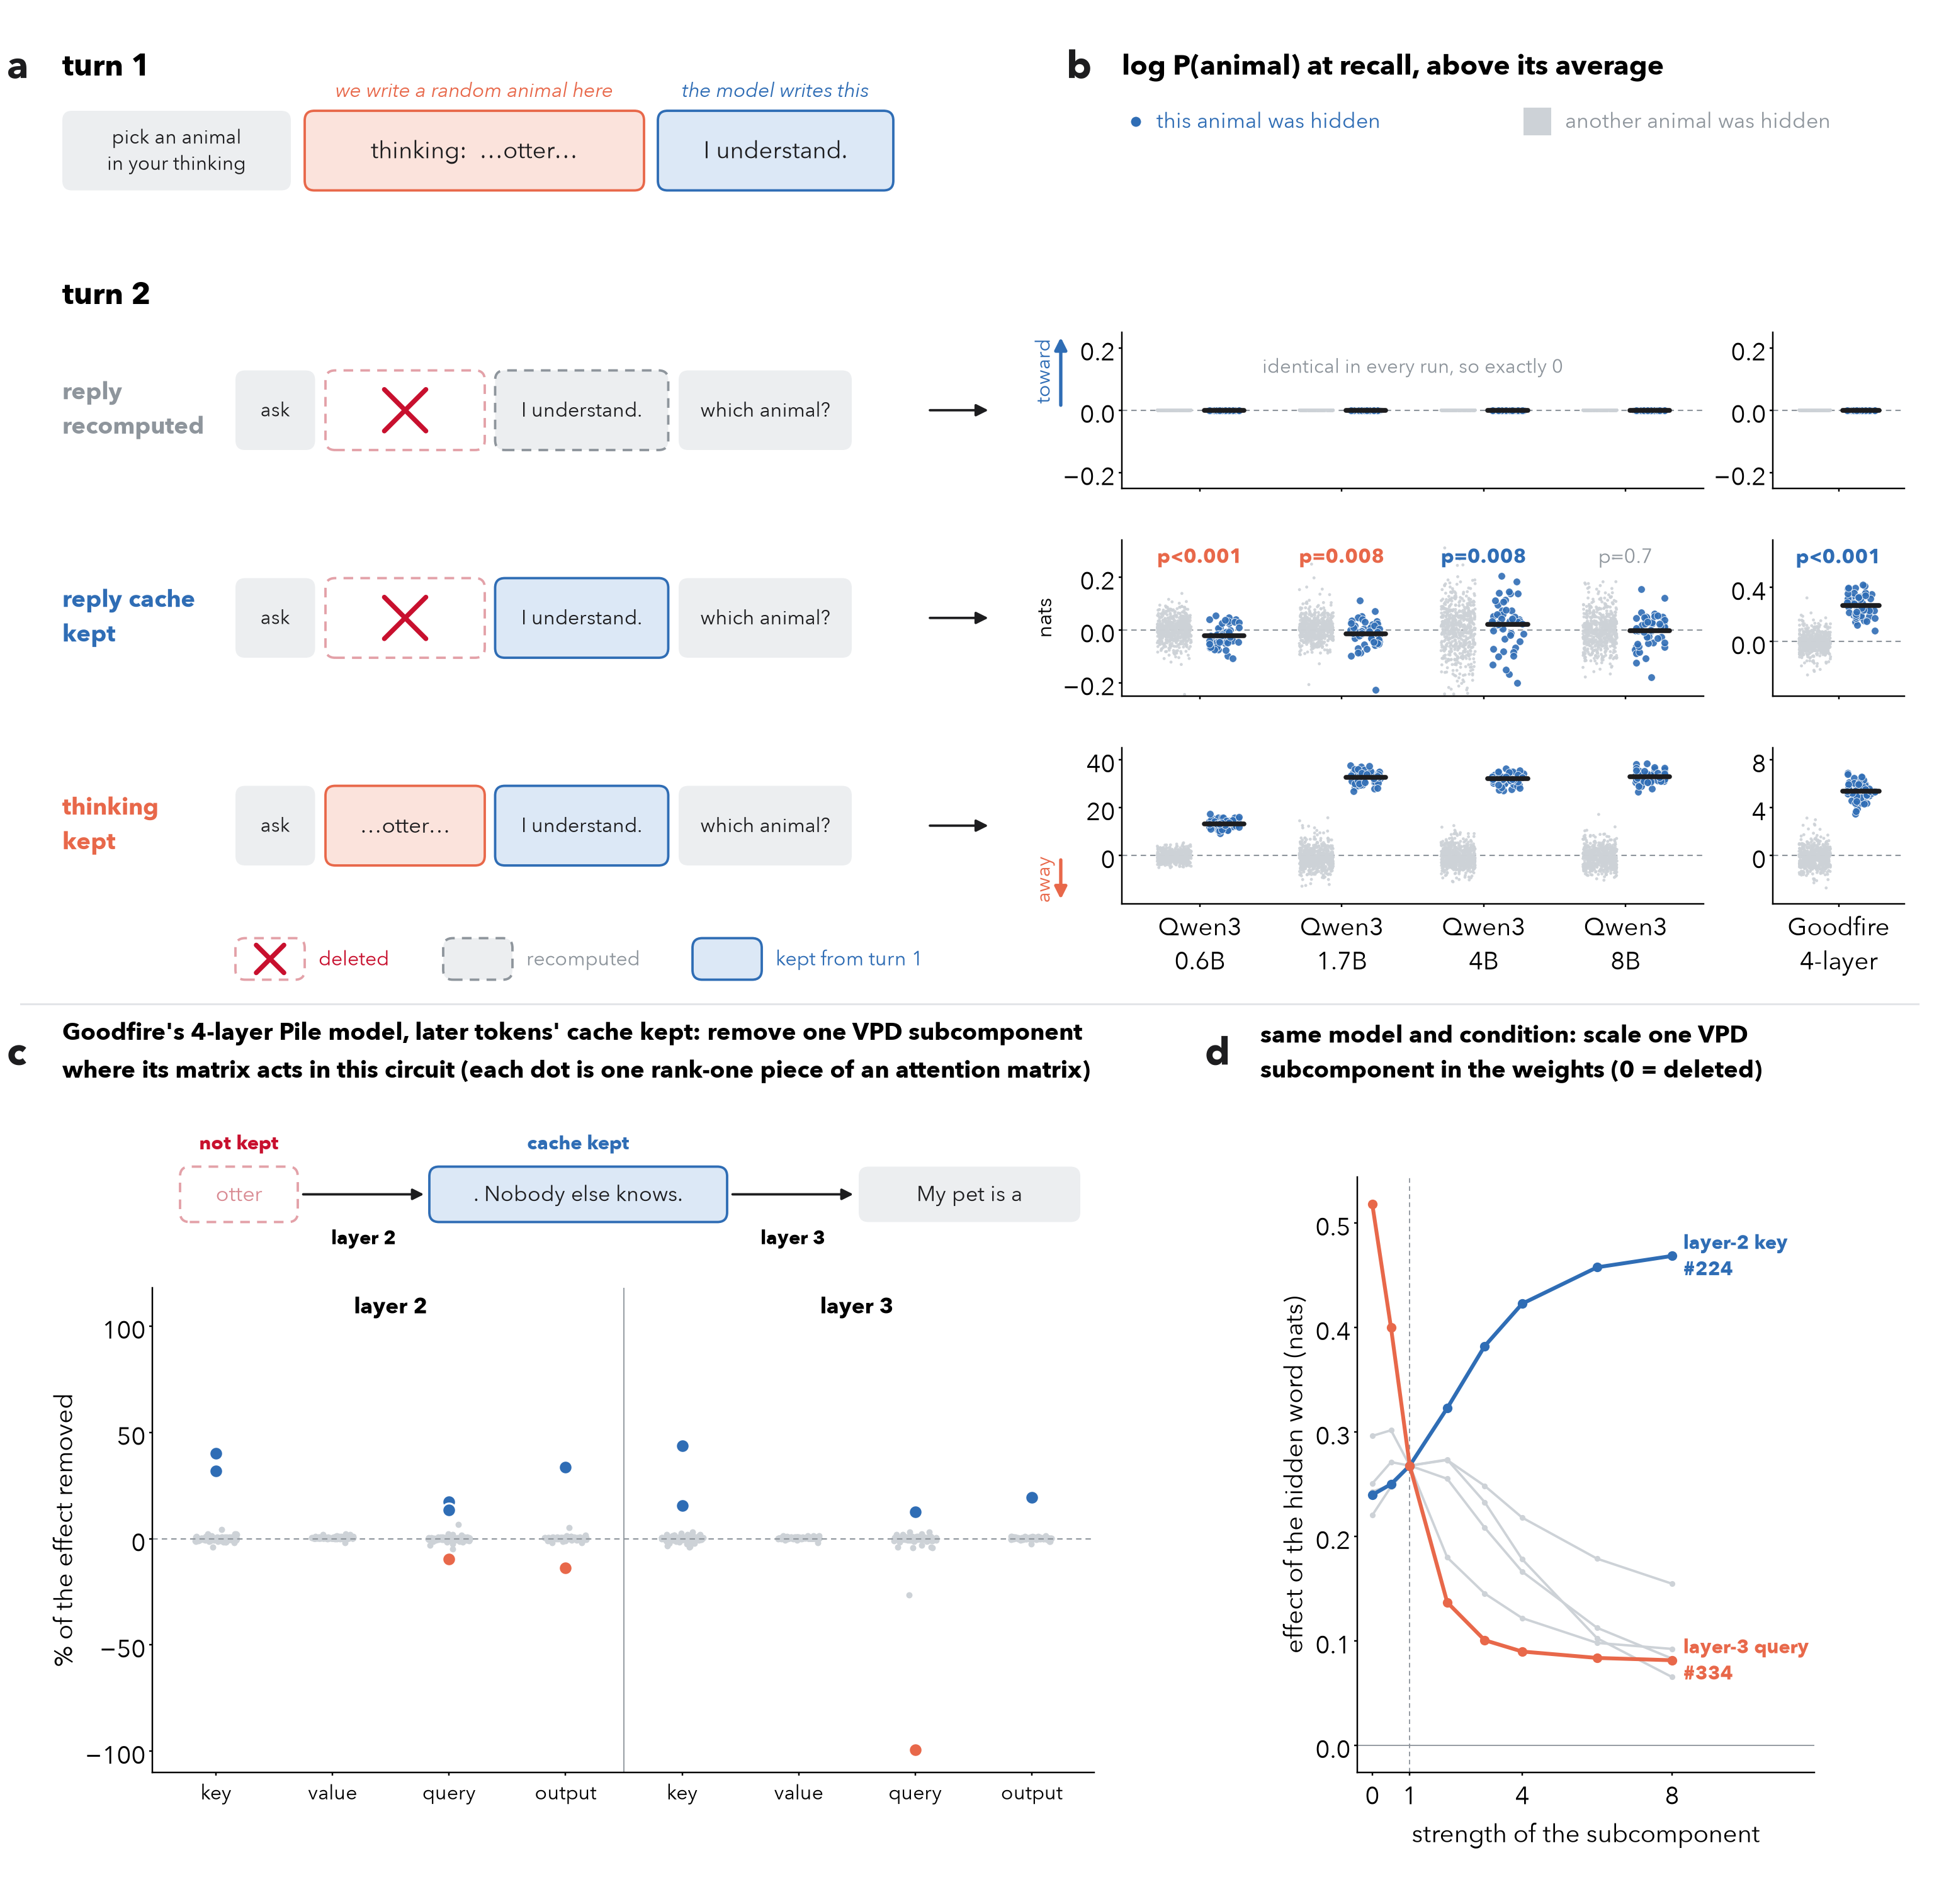
\includegraphics[width=\linewidth]{figs/main.png}
\caption{\textbf{a}, the task: we write a random animal into the thinking; the model writes the rest and replies. In turn
2 the cache holds the reply recomputed without the thinking, the reply's turn-1 keys and values (the thinking's entries
deleted), or the thinking itself. \textbf{b}, for each model and condition, the log-probability of each animal at
recall in the runs where it was the hidden animal (blue; one point per animal, bar = mean) or where another animal was
hidden (gray), minus its average over all runs; p-values from the two-sided animal-level permutation test, colored by
the direction of the effect. The last column runs the same three conditions as plain text on Goodfire's 4-layer
model. \textbf{c}, in that model, with the later tokens' cache kept and the word not kept: the share of the effect
removed by deleting one VPD subcomponent. \textbf{d}, the effect when one subcomponent of the weights is scaled
($W \to W + (a-1)uv^\top$).}
\label{fig:main}
\end{figure}

\section{Setup}

\paragraph{Task.} Turn 1 lists 50 animals and asks the model to choose one in its thinking, hold it in mind, and reply
with exactly ``I understand.''. For each run an animal $c$ is drawn uniformly from the 50 and written at the start of
the thinking (``\texttt{Draw \#$n$: $c$. \dots\ I'll keep $c$ in mind.}'', with one of six opening and seven closing
sentences and a random three-digit $n$, so that no two runs share a context); the model writes the rest of the thinking
and the reply (temperature 0.6, top-$p$ 0.95, top-$k$ 20). Runs whose visible reply is exactly ``I understand.'' are
kept (96--100\%). Turn 2 asks which animal was chosen. Drawing the animal uniformly, instead of letting the model choose,
removes the model's preferences among animals from the comparison: under the null hypothesis that turn 2 carries no
information about turn 1, every animal is equally likely to be the hidden one in every context. Two wordings of both
turns are used (Appendix~\ref{app:prompts}); a version in which the model chooses freely is reported in
\pending{section}.

\paragraph{Conditions.} Turn 2 is read with three contexts that differ only in what stands for turn 1's assistant
message (Figure~\ref{fig:main}a):
\begin{itemize}
\item \emph{reply recomputed}: the reply's keys and values are computed without the thinking. Every run's turn-2
context is then the same token sequence with the same cache, so the hidden animal cannot affect the answer.
\item \emph{reply cache kept}: the reply's keys and values are those computed in turn 1, with the thinking present. The
thinking's own entries are deleted, and the reply's keys are rotated back by $T$ positions ($T$ the thinking's length)
so that the reply occupies the same positions as when recomputed. Values carry no position and are kept as computed.
\item \emph{thinking kept}: the thinking stays in context (a positive control).
\end{itemize}
A fourth condition keeps the reply cache but asks in turn 2 for any animal from the list, to separate a priming of the
hidden animal from an answer to the question (Appendix~\ref{app:neutral}).

\paragraph{Readout.} After turn 2 the model is given an empty thinking block and the text ``\texttt{Animal:}''. For
run $i$ and animal $b$, $L_{ib}$ is the log-probability that the continuation is $b$'s name (the log of the summed
probabilities of its capitalized and lower-case forms, each a full multi-token sequence).

\paragraph{Statistics.} For animals $a$ and $b$, $M_{ab}$ is the mean of $L_{ib}$ over the runs whose hidden animal is
$a$, minus the mean of $L_{ib}$ over all runs; Figure~\ref{fig:main}b plots the diagonal of $M$ (blue) and its
off-diagonal entries (gray). The test statistic is the mean of the diagonal of $M$ after its row and column means are
removed; its null distribution re-pairs rows with columns by uniformly random permutations (20{,}000 draws), the
two-sided $p$ is the share of draws at least as far from the null mean, and $z$ is the distance from the null mean in
null standard deviations. Runs that share an animal share part of their context, so runs are not exchangeable under
the null, while animals are: a test that permutes runs gave $p<0.05$ in 15--28\% of placebo relabellings of the
animals, and the animal-level test in \pending{x}\% (nominal 5\%; Appendix~\ref{app:calibration}). For the heads and
mechanisms of Section~\ref{sec:mech}, heads are selected on one run (the discovery seed) and every claim is tested on a
second run with a different seed (the confirmation seed).

\section{Results}

\subsection{The hidden animal shifts the recall answer only through the reply's cache}
\pending{Figure 1b: per model, discovery and confirmation; 0.6B, 1.7B, 4B, 8B; wording A and B; neutral question;
free choice; visible control. Top-1 at chance everywhere.}

\subsection{Qwen3-1.7B reads it in layer 21}\label{sec:mech}
\pending{bands, reply tokens, every key/value head; promoter 21:0 and suppressors 21:5, 21:6 in both wordings; the
suppressor 21:6 attends to the reply 4x more under wording A and its single-head effect is 2.2x larger, which reverses
the net sign; keys and values both required; the direct path is a minority of the effect; the three heads combine
non-additively; the animal is spread over many value directions; no single turn-1 layer writes it; dose-response.}

\subsection{What the weights of those heads say, and where that stops}
\pending{weights-only copying score has the sign of each head's effect in this task; on ordinary text, removing the
heads does not change repeated tokens in the direction the copying score predicts (correlation +0.19 over 80 heads in
layers 18--27).}

\subsection{The same route in a 4-layer model with a parameter decomposition}
\pending{text version: stripped 0, retained +0.27 nats (z 28.6), visible +5.4; route: layer 2 copies the word into
the later tokens, layer 3 reads it at the cue; VPD subcomponent deletions as weight edits; MLP subcomponents in layers
0--1 at the word; weight-edit dose curves (query \#334: 0.52 deleted, 0.27, 0.08 at 8x; key \#224: 0.47 at 8x); scaling
the later tokens' word-dependent cache restores naming (2\% to 64\% at 8x) while no single subcomponent does.}

\section{Limitations}
\pending{forced choice; one task and two wordings; serving setups that keep the reply cache; Qwen3 only plus one
4-layer model; the decomposition's subcomponents are a basis for edits, not a proof of mechanism.}

\appendix
\section{Prompts}\label{app:prompts}
\pending{both wordings verbatim}
\section{Priming control}\label{app:neutral}
\pending{neutral question results}
\section{Calibration}\label{app:calibration}
\pending{placebo results}

\end{document}
